\documentclass[preprint,12pt]{elsarticle}

\usepackage[T1]{fontenc}
\usepackage[utf8]{inputenc}
\usepackage{newtxtext,newtxmath}
\usepackage[ruled,vlined]{algorithm2e}
\usepackage{array}
\usepackage{booktabs}
\usepackage[final]{microtype}
\usepackage{graphicx}
\usepackage{hyperref}
\usepackage{longtable}
\usepackage{multirow}
\usepackage{ragged2e}
\usepackage{tabularx}
\usepackage{url}

\journal{Preprint prepared for arXiv}
\hypersetup{hidelinks}
\setlength{\emergencystretch}{2em}
\setlength{\textfloatsep}{7pt plus 2pt minus 2pt}
\setlength{\dbltextfloatsep}{7pt plus 2pt minus 2pt}
\setlength{\floatsep}{5pt plus 2pt minus 2pt}
\setlength{\intextsep}{5pt plus 2pt minus 2pt}
\setlength{\abovecaptionskip}{4pt}
\setlength{\belowcaptionskip}{1pt}
\renewcommand{\arraystretch}{0.88}
\newcolumntype{Y}{>{\RaggedRight\arraybackslash}X}
\newcolumntype{P}[1]{>{\RaggedRight\arraybackslash}p{#1}}

\begin{document}

\begin{frontmatter}

\title{Beyond Direct Correction: A Rule-Tool and LLM Hybrid Framework for Multi-Dimensional Feedback in High School English Writing}

\author{Anonymous Author}
\address{Draft prepared in April 2026}

\begin{abstract}
LLM-based writing support often improves drafts more readily than it supports revision. This paper tests whether a rule-tool and large language model hybrid can instead deliver pedagogically structured feedback for high school English writing under reproducible benchmark conditions. The framework combines rule-grounded local diagnosis with a four-layer scaffold of diagnosis, hint, strategy, and exemplar across grammar, vocabulary, organization, and coherence. On fixed subsets of Feedback Prize ELL and ASAP-AES, \textit{Hybrid} improves pedagogical depth over direct feedback for \texttt{GPT-5.4-mini} but not for \texttt{DeepSeek v3.2} or \texttt{GLM-5}. Across models, however, it remains clearly safer than direct rewrite, and structured outputs stay valid enough for matched comparison. Failure-focused prompt tightening further improves depth and preservation on difficult \texttt{GPT-5.4-mini} cases. The results therefore support the hybrid premise only in qualified form: its benefits are model-dependent and remain bounded by benchmark-proxy evaluation rather than classroom outcomes.
\end{abstract}

\begin{keyword}
high school English writing \sep pedagogical feedback \sep large language models \sep rule-based diagnosis \sep formative assessment
\end{keyword}

\end{frontmatter}

\section{Introduction}

Large language models are increasingly used for tutoring, assessment, and writing support in English education \cite{ye2025position}. In secondary-school writing, however, their most accessible use case is still direct correction: a student submits a draft and receives a cleaner version. That behavior can improve text quality while weakening the revision process the learner is meant to practice. Pedagogically useful assistance should instead help students recognize problems, attempt revision, and retain ownership of the draft.

Existing work leaves three gaps. First, many systems optimize immediate text improvement rather than guided revision. Second, support is uneven across writing dimensions: rule tools and grammar-focused prompting help with local errors, but vocabulary precision, organization, and coherence still depend on broader discourse judgment. Third, pedagogical claims remain hard to compare when prompting, task scope, and output format vary across studies, leaving benchmark-based evaluation under-specified \cite{ye2025position,jaganov2025dynamic}.

We address these gaps with \textit{Hybrid}, a rule-tool and LLM framework that anchors local evidence while generating four-layer feedback across grammar, vocabulary, organization, and coherence. The paper makes three contributions: it formulates high school writing support as guided revision rather than direct substitution; it implements a hybrid design that combines stable surface diagnosis with discourse-level LLM guidance; and it evaluates that design on public learner-writing datasets using matched pedagogical, preservation, schema-validity, and blinded human metrics.

The paper therefore asks whether structured hybrid feedback improves on direct feedback without giving up authorship preservation, whether its coverage extends across local and discourse dimensions, and whether any gains survive cross-model comparison. Its claim is deliberately narrow: the reported evidence concerns feedback form, safety, and robustness on public benchmark proxies, not classroom learning outcomes.

\section{Related Work}

\subsection{Automated Writing Evaluation and Diagnostic Feedback}

Automated support for student writing has a long trajectory rooted in rule-based diagnostics and rubric-aligned trait analysis. Systems such as Criterion linked handcrafted linguistic features to scoring rubrics and returned interpretable error annotations to both students and teachers \cite{burstein2004criterion}. Validity-oriented frameworks later formalized the relationship between diagnostic constructs and assessment inferences, treating transparency as a design requirement rather than a post hoc property \cite{chapelle2015validity,weigle2002assessing}. Writing Mentor extended this line by targeting self-regulated revision in struggling writers through structured, trait-level prompts \cite{madnani2018writing}. The shared strength of these systems is inspectability: error categories, rubric constructs, and feedback rationales remain visible to instructors and amenable to principled evaluation.

That inspectability, however, is tightly coupled to local surface evidence. Grammar, spelling, and a narrow set of usage patterns can be diagnosed reliably, but vocabulary precision, rhetorical organization, and inter-sentential coherence lie largely outside the reach of hand-authored rule sets. As a result, traditional AWE systems offer strong local control at the cost of uneven dimensional coverage---a limitation that becomes consequential when the pedagogical goal is guided revision across multiple writing dimensions rather than surface correction alone. The gap between local diagnostic strength and discourse-level guidance motivated the adoption of learned representations in subsequent work.

\subsection{Neural Scoring and Sequence-Level Correction}

Neural methods reframed writing evaluation as representation learning, replacing handcrafted features with distributed encodings of essay quality. Survey work on automated essay scoring documents the shift from feature-engineering pipelines to recurrent and attention-based architectures trained end-to-end on holistic or trait-level scores \cite{ke2019aes}. Early neural AES models demonstrated that learned representations can match or exceed earlier pipelines on benchmark datasets such as ASAP \cite{taghipour-ng-2016-neural}. In parallel, neural approaches to grammatical error correction recast the task as low-resource machine translation or sequence labeling, achieving substantial gains over statistical baselines \cite{junczysdowmunt2018approaching}. Sequence-tagging formulations such as GECToR further improved inference efficiency by replacing autoregressive decoding with parallel token-level edits \cite{omelianchuk-etal-2020-gector}, and instruction-tuned editing models like CoEdIT extended controllable rewriting to diverse text-editing intents \cite{raheja2023coedit}.

These advances improved both scoring accuracy and correction fluency. Learned representations capture discourse-level regularities that rule-based features miss, and sequence-editing architectures reduce the latency and error-propagation costs of autoregressive generation. Yet the optimization targets of this family---scores, corrected tokens, or fluency-edited outputs---remain oriented toward improving the text artifact rather than supporting the student's revision process. A model that returns a higher score or a cleaner sentence does not by itself make the underlying problem visible, suggest a transferable strategy, or calibrate the amount of help to what the learner can use. The pedagogical gap between better output and better guidance remained largely unaddressed until generative language models opened a different design space.

\subsection{LLM-Based Writing Support and Feedback Generation}

Large language models introduced the possibility of generating discursive, multi-dimensional feedback rather than returning scores or local edits alone. Position analyses and survey work on LLMs in English education document their potential as tutors that can adapt register, explain errors, and model revision strategies \cite{ye2025position,chu2025agents}. Empirical studies in EFL and L2 contexts show that LLMs can produce feedback that is more detailed and fluent than instructor baselines under controlled conditions \cite{dai2023feedback,han2024llm}, while dynamic-assessment designs demonstrate that model-mediated interaction can approximate graduated scaffolding for grammatical accuracy \cite{jaganov2025dynamic}. Comparative evaluations further clarify the boundary: trained human raters still outperform ChatGPT on prioritization, accuracy, and supportive tone for secondary-level essays, though the practical differences are modest enough to make LLM feedback a viable supplement \cite{steiss2024comparing}. Framework-level efforts such as SEFL formalize synthetic feedback generation with multi-agent pipelines, moving the field toward reproducible, schema-driven output \cite{zhang2025sefl}. Separately, the feedback comment generation shared task introduced the problem of producing explanatory notes for marked learner-text spans, framing pedagogical commentary as a structured generation task distinct from correction \cite{nagata2021fcg}.

The breadth of this work confirms that LLMs can say substantially more than earlier systems. The unresolved issue is whether that generative flexibility can be reliably constrained. Without structural control, the same capacity that enables richer commentary also enables over-rewriting, unstable output schemas, and prompt-specific behavior that resists fair comparison. Studies that demonstrate feedback quality under one prompt or one model do not necessarily transfer to matched multi-condition evaluation, and few existing designs simultaneously test pedagogical depth, student-text preservation, and structured-output reliability within a single protocol.

\subsection{Learner-Writing Benchmarks and Evaluation Protocols}

Public benchmarks supply the controlled data needed to make the above concerns testable. ASAP-AES provides holistic writing-quality scores across multiple prompts and grade levels. Feedback Prize ELL offers analytic trait annotations---cohesion, syntax, vocabulary, phraseology, grammar, and conventions---on English language learner essays. BEA-2019 standardized grammatical error correction evaluation with shared test sets and scorer software \cite{bryant2019bea}. Together, these resources cover complementary aspects of learner writing: holistic quality, trait-level analysis, and local correction.

Benchmarks alone, however, do not specify how pedagogical feedback should be structured, compared, or validated. Existing evaluation protocols either target a single output type---a score, a corrected sentence, or a generated comment---or rely on classroom evidence that is expensive to replicate at scale. The result is a protocol gap: rich feedback frameworks lack matched benchmark evaluation, and benchmark-oriented studies lack pedagogical depth metrics. Schema-validity work on structured LLM outputs demonstrates that generation reliability can itself be measured \cite{geng2025jsonschemabench}, but this capability has not yet been integrated into writing-feedback evaluation pipelines.

The gap that emerges from the preceding lines of work is therefore not primarily architectural but evaluative: no existing protocol combines rule-grounded local diagnosis, layered pedagogical scaffolding, ownership-preservation measurement, and cross-model benchmark comparison within a single matched design. \textit{Hybrid} is positioned at that intersection. It uses stable surface diagnostics to anchor a four-layer feedback scaffold, extends guidance across grammar, vocabulary, organization, and coherence, and evaluates the result on public learner-writing corpora under matched conditions---so that feedback quality, structured-output reliability, and student-text preservation can be assessed together rather than in isolation.

\section{Hybrid Pedagogical Feedback Framework}

\subsection{Theoretical Anchoring}

The four-layer design follows a minimal instructional progression rather than prompt convenience alone. The \textit{Hint} layer reflects the idea that feedback should provide only the support needed for an initial revision attempt \cite{vygotsky1978mind}. The ordered movement from \textit{Diagnosis} to \textit{Hint}, \textit{Strategy}, and \textit{Exemplar} is consistent with graduated assistance and with the distinction between immediate task information and process-level guidance \cite{aljaafreh1994negative,hattie2007power}. The resulting ordering operationalizes the paper's main pedagogical premise: guidance should support revision before it replaces it.

\begin{table}[t]
\centering
\scriptsize
\caption{Four-layer feedback structure.}
\begin{tabularx}{\linewidth}{@{}P{0.15\linewidth}P{0.38\linewidth}Y@{}}
\toprule
Layer & Operational function & Pedagogical role \\
\midrule
Diagnosis & Locate and name the problem. & Makes the issue visible. \\
Hint & Provide a cue without fully solving it. & Supplies minimal scaffold. \\
Strategy & State a reusable revision principle. & Transfers beyond one local fix. \\
Exemplar & Show a short local revision. & Models a move without replacing the draft. \\
\bottomrule
\end{tabularx}
\end{table}

\subsection{Problem Definition}

We formulate the task as benchmark-based pedagogical feedback generation for high school English writing. Given a student essay $x$ from a public learner-writing resource, the system produces a feedback record $y$ rather than a rewritten essay. The target object is revision support across grammar, vocabulary, organization, and coherence, and in the main structured setting $y$ contains \textit{diagnosis}, \textit{hint}, \textit{strategy}, and \textit{exemplar}. Two constraints distinguish the task from generic rewriting: feedback should preserve student authorship, and outputs should be standardized enough for fair comparison across conditions.

\subsection{Pipeline Overview}

Figure~\ref{fig:framework_overview} and Algorithm~\ref{alg:hybrid_pipeline} make the execution order explicit. The key design decision is to separate evidence anchoring, pedagogical generation, and post-generation normalization so that the same essay can be compared across conditions without changing the shared storage schema.

\begin{figure*}[!t]
\centering
\makebox[\textwidth][c]{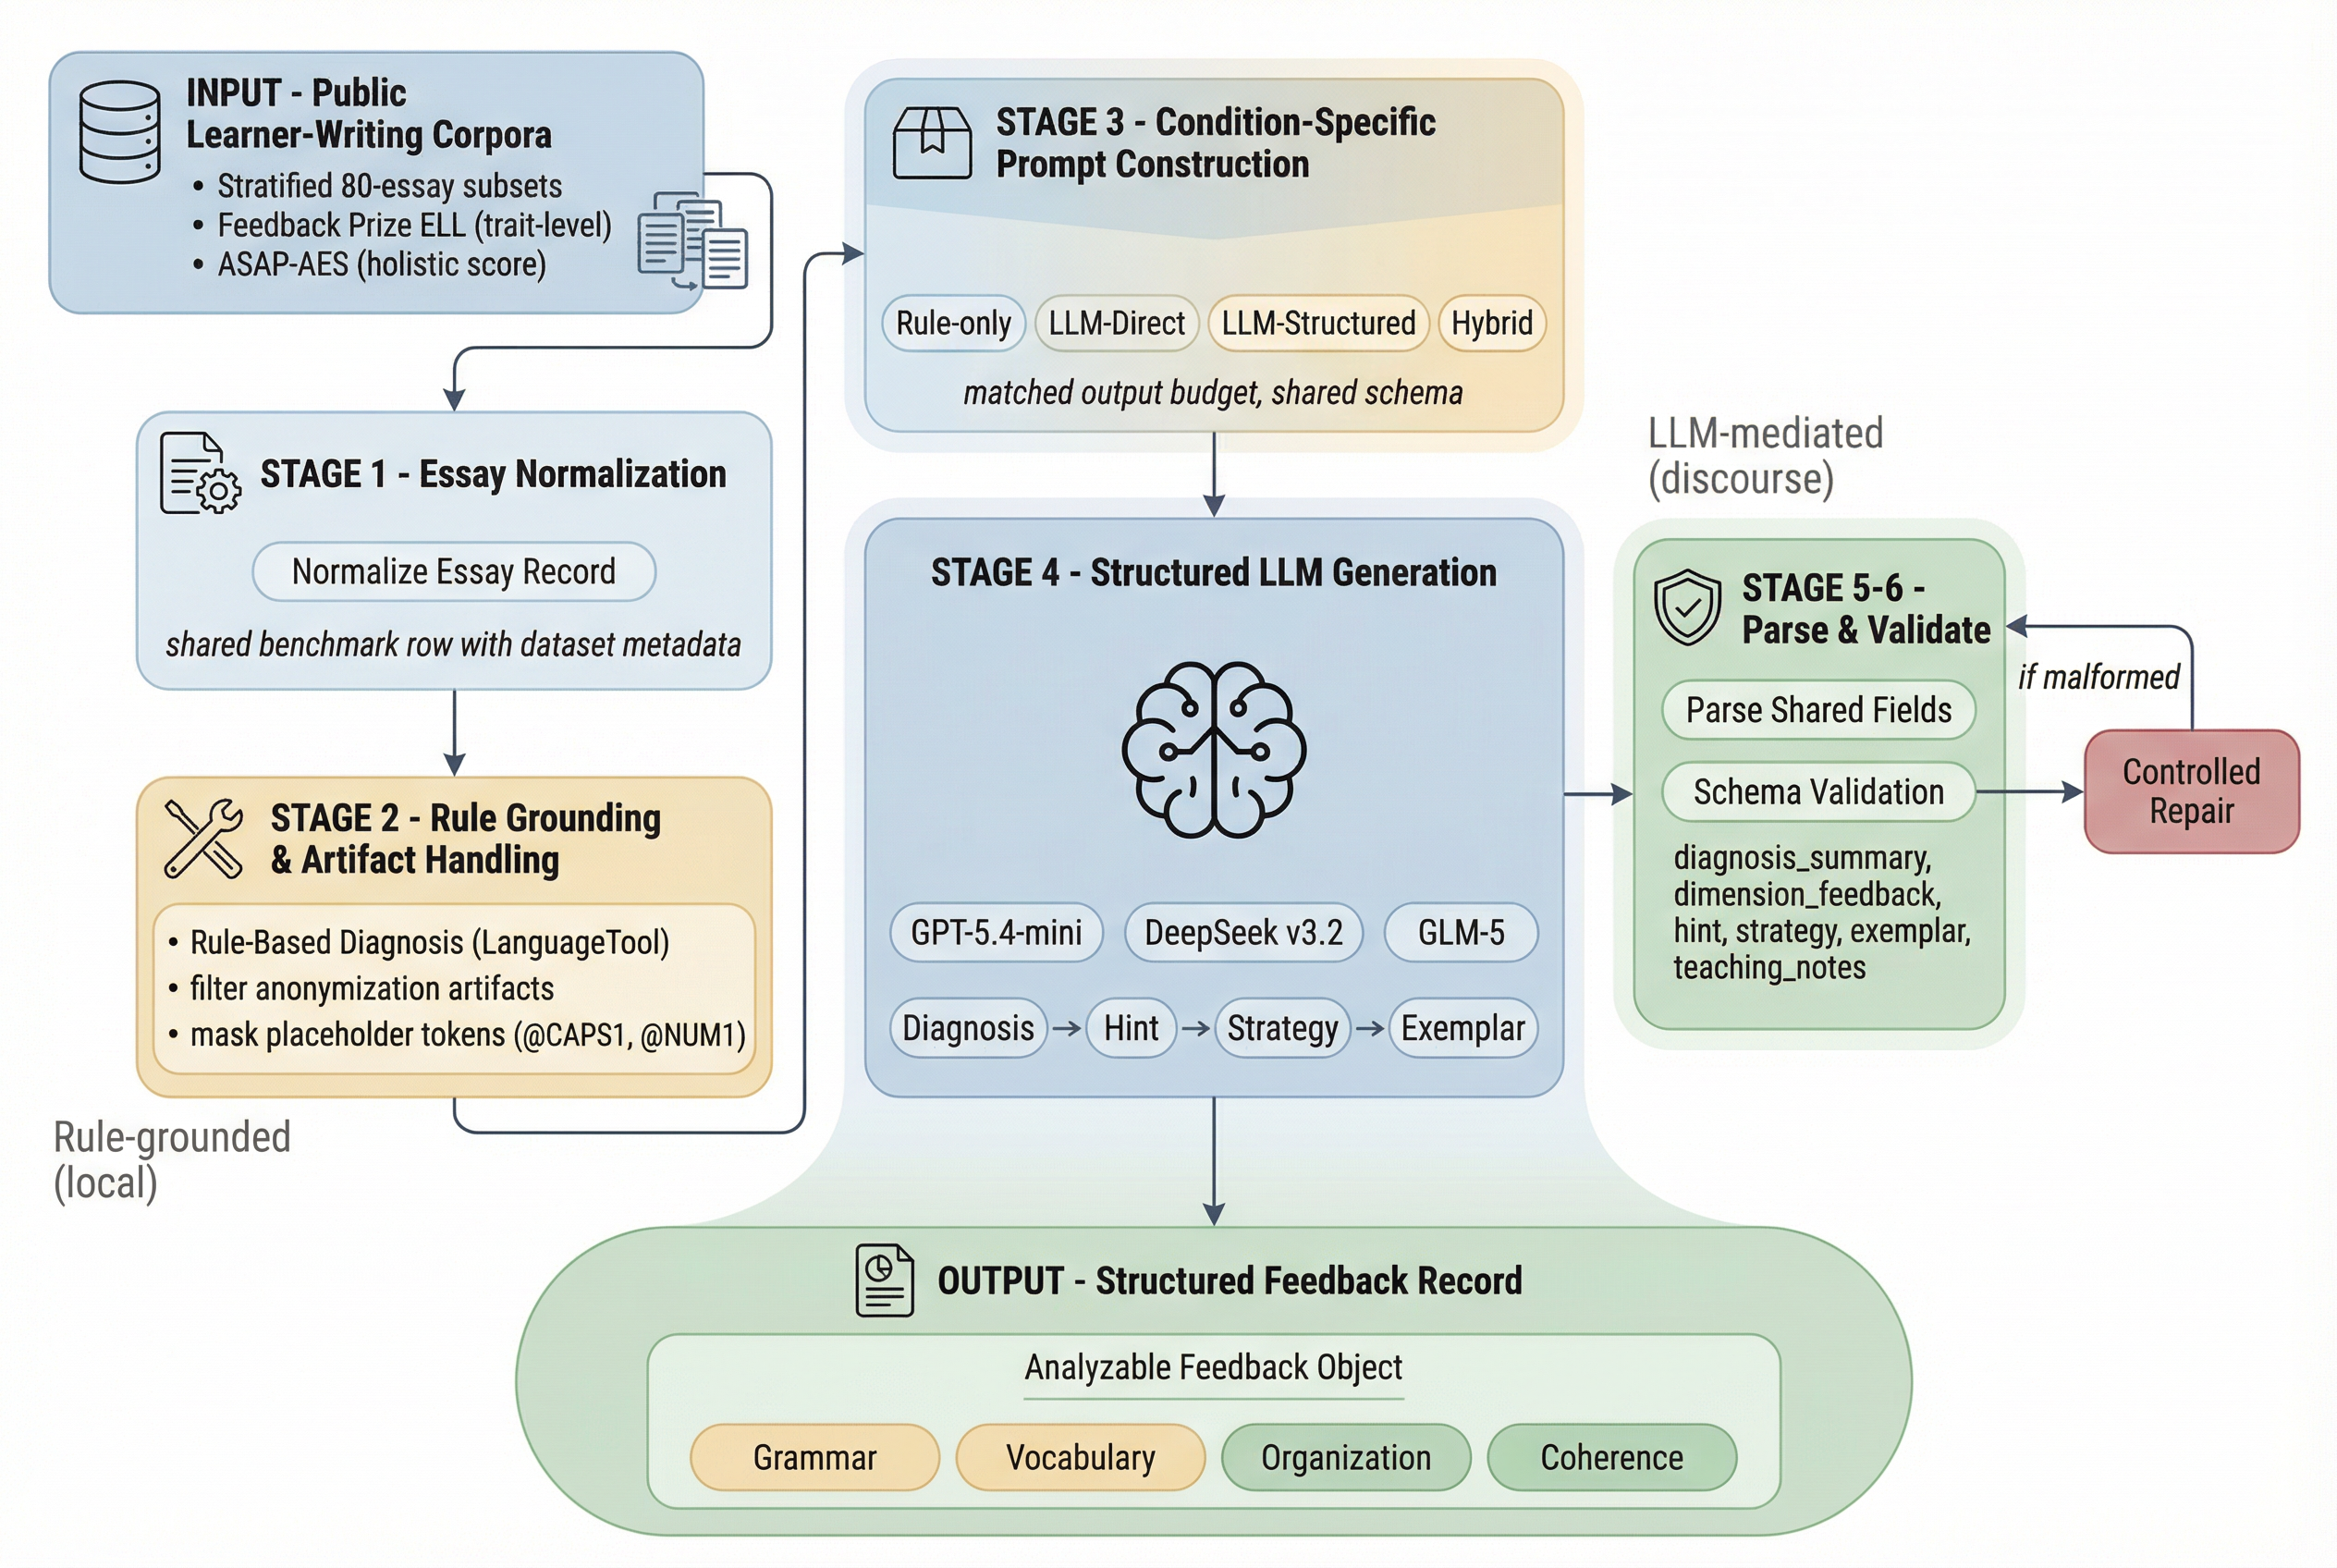
\includegraphics[width=1.08\textwidth]{Fig/figure1_hybrid_framework_cell_final_cropped.png}}
\caption{Stage-level overview of the rule-tool and LLM hybrid framework. The pipeline normalizes public learner-writing records, anchors local evidence with rule-based diagnosis and artifact filtering, builds condition-specific prompts under a shared schema, generates layered feedback, and then parses, validates, and selectively repairs outputs before returning an analyzable feedback object across grammar, vocabulary, organization, and coherence.}
\label{fig:framework_overview}
\end{figure*}

\begin{algorithm}[H]
\SetKwInOut{Input}{Input}\SetKwInOut{Output}{Output}
\SetKwProg{Fn}{Function}{}{}
\SetKwFunction{NormalizeEssayRecord}{NormalizeEssayRecord}
\SetKwFunction{RunRuleDiagnosis}{RunRuleDiagnosis}
\SetKwFunction{BuildPromptPackage}{BuildPromptPackage}
\SetKwFunction{GenerateStructuredFeedback}{GenerateStructuredFeedback}
\SetKwFunction{ParseSharedFields}{ParseSharedFields}
\SetKwFunction{ValidateSchema}{ValidateSchema}
\SetKwFunction{RepairIfNeeded}{RepairIfNeeded}
\SetKwFunction{HybridPipeline}{HybridPipeline}
\small
\caption{\textit{Hybrid} pipeline for pedagogical feedback generation}
\label{alg:hybrid_pipeline}
\Input{essay text $x$; feedback condition $c$; output-budget configuration $\mathcal{B}$; optional rule engine $\mathcal{R}$}
\Output{structured feedback record $y$; validation metadata $v$}
\Fn{\HybridPipeline{$x,c,\mathcal{B},\mathcal{R}$}}{
\tcp{Stage 1: Shared essay normalization}
$r \leftarrow \NormalizeEssayRecord(x)$\tcp*{shared benchmark row with dataset metadata}
\tcp{Stage 2: Rule grounding and artifact handling}
$(d,m) \leftarrow \RunRuleDiagnosis(r,\mathcal{R})$\tcp*{filter anonymization artifacts and mask placeholder tokens}
\tcp{Stage 3: Condition-specific prompt construction}
$p \leftarrow \BuildPromptPackage(r,d,m,c,\mathcal{B})$\tcp*{same schema, matched budget, condition-specific evidence}
\tcp{Stage 4: Structured LLM generation}
$\tilde{y} \leftarrow \GenerateStructuredFeedback(p)$\tcp*{JSON-targeted generation under the shared schema}
\tcp{Stage 5: Parse into shared fields}
$y \leftarrow \ParseSharedFields(\tilde{y})$\tcp*{diagnosis\_summary, dimension\_feedback, hint, strategy, exemplar, teaching\_notes}
\tcp{Stage 6: Schema validation}
$v \leftarrow \ValidateSchema(y,r,\mathcal{B})$\tcp*{completeness, label consistency, layer presence, exemplar budget}
\tcp{Stage 7: Controlled failure-path repair}
\If{$y$ is empty or malformed}{
$(y,v) \leftarrow \RepairIfNeeded(\tilde{y},r,c,\mathcal{B},v)$\tcp*{repair only on failure paths and keep the trace}
}
\tcp{Stage 8: Return analyzable feedback object}
\Return{$y,\ v$}\;
}
\end{algorithm}

The pipeline separates evidence anchoring, condition-specific generation, and post-generation validation so that the same essay can be compared under a shared schema. Each essay--condition pair uses one rule pass, one main generation call, and repair only on failure paths, which keeps the benchmark tractable while making failures inspectable.

\subsection{Operationalizing the Four Writing Dimensions}

The benchmark fixes four target dimensions. Grammar and vocabulary are mostly local, although vocabulary still requires LLM judgment beyond spelling or form alerts. Organization and coherence are discourse-level dimensions handled primarily by the LLM layer. This split motivates the division of labor in the framework: rule evidence anchors local issues, while the model extends feedback to broader rhetorical and flow-related problems.

\subsection{Schema, Feedback Granularity, and Conflict Policy}

The shared record contains \texttt{diagnosis\_summary}, \texttt{dimension\_feedback}, \texttt{hint}, \texttt{strategy}, \texttt{exemplar}, and \texttt{teaching\_notes}. To keep conditions comparable, each essay may include at most five issue clusters, each dimension may contribute at most two short comments, and exemplars are capped at 15\% of source length in the four main conditions. Rule evidence is advisory rather than binding: the LLM may add organization or coherence guidance when the rule layer is silent and may downgrade likely false positives, but it may not invent rule hits. Placeholder tokens such as \texttt{@CAPS1} and \texttt{@NUM1} are filtered as artifacts rather than treated as learner errors.

\subsection{Comparison Conditions and Fairness Controls}

The benchmark compares \textit{Rule-only}, \textit{LLM-direct-feedback}, \textit{LLM-structured}, and \textit{Hybrid} under matched output budgets and student-facing prompts. A supplementary \textit{LLM-direct-rewrite} condition is retained only as a negative control for overwrite analysis and is not included in the main benchmark table. The shared schema and matched budgets are intended to keep condition differences attributable to feedback design rather than output length or storage format.

\section{Datasets and Experimental Setup}

\subsection{Public Data Resources}

The main benchmark uses two public Kaggle corpora: Feedback Prize ELL (\href{https://www.kaggle.com/competitions/feedback-prize-english-language-learning}{official page}) for trait-level learner-writing analysis and ASAP-AES (\href{https://www.kaggle.com/competitions/asap-aes}{official page}) for holistic essay quality. Both are treated as reproducible learner-writing proxies rather than classroom outcome data. For each model, we report fixed stratified subsets of 80 essays per dataset, plus 10 direct-rewrite supplementary cases per dataset for overwrite analysis.

\subsection{Research Questions}

\begin{itemize}
    \item \textbf{RQ1}: Does \textit{Hybrid} improve pedagogical usefulness over \textit{LLM-direct-feedback} without substantial correction loss?
    \item \textbf{RQ2}: Does \textit{Hybrid} provide more balanced grammar, vocabulary, organization, and coherence coverage than \textit{Rule-only} and \textit{LLM-structured}?
    \item \textbf{RQ3}: Does \textit{Hybrid} preserve more student-authored text than direct rewrite, and can tighter exemplar control narrow the gap to direct feedback?
    \item \textbf{RQ4}: Are hybrid gains stable across models of different strength, or are they highly model-dependent?
\end{itemize}

\subsection{Benchmark Scope and Dataset--Task Alignment}

The reported results intentionally stay within this proxy setting. They test whether a feedback framework can produce structured, pedagogically legible, and ownership-preserving outputs on public learner corpora; they do not establish learning gain, tutoring interaction quality, or ecological fit to Chinese high-school classrooms.

\subsection{Models and Reproducibility Controls}

The executed comparison uses three OpenRouter-accessible models: \texttt{deepseek/deepseek-chat}, \texttt{openai/gpt-5.4-mini}, and \texttt{z-ai/glm-5}.\footnote{Execution-time access identifiers are reported as logged rather than anonymized aliases.} For readability, we refer to them as \texttt{DeepSeek v3.2}, \texttt{GPT-5.4-mini}, and \texttt{GLM-5}. All runs use the same prompt family, temperature and \texttt{top\_p} settings, token budget, LanguageTool-compatible diagnosis layer, request caching, and resumable batch execution so that within-model condition contrasts remain matched.

\subsection{Automatic Evaluation}

Automatic evaluation covers correction-oriented metrics where available, trait or holistic proxies on the essay datasets, and schema-validity checks for structured generation. Pedagogical usefulness is operationalized through actionability, clarity, dimension coverage, non-overwriting, student-text preservation, and learner-autonomy support; pedagogical depth combines these components with weights 0.30, 0.20, 0.25, 0.15, and 0.10 respectively for actionability, clarity, coverage, non-overwriting, and scaffolding bonus. Because the framework depends on structured outputs, we also track JSON parse success, field completeness, dimension-label consistency, and layer presence \cite{geng2025jsonschemabench}. Bootstrap intervals, weight-perturbation checks, and full formulas are reported in the supplementary material and released code.

\subsection{Rater-Based Evaluation}

The reported human review is a blinded two-rater check on 24 sampled items from the three conditions prioritized in the main results table: direct feedback, hybrid, and rule-only. Raters with EFL teaching or writing-assessment backgrounds score actionability, clarity, pedagogical usefulness, dimension coverage, rewrite safety, and learner-autonomy support on 1--5 scales using a shared guide. Agreement is reported with quadratic weighted kappa.

\section{Results}

\subsection{Main Results}

Table~\ref{tab:main_results} reports the completed low-token cross-model run on the fixed ELL and ASAP subsets. All models use the same prompt family and cached execution, and the direct-rewrite supplement is used only for overwrite analysis.

\begin{table}[t]
\centering
\scriptsize
\caption{Cross-model low-token results on ELL and ASAP-AES. Delta is \textit{Hybrid} minus \textit{LLM-direct-feedback} on pedagogical depth.}
\label{tab:main_results}
\begin{tabular*}{\linewidth}{@{\extracolsep{\fill}}llccccc@{}}
\toprule
Dataset & Model & Direct depth & Hybrid depth & Delta & Direct preserv. & Hybrid preserv. \\
\midrule
\multirow{3}{*}{ELL} & \texttt{GPT-5.4-mini} & 0.7603 & 0.7755 & +0.0152 & 0.9525 & 0.9212 \\
 & \texttt{DeepSeek v3.2} & 0.8233 & 0.7714 & -0.0519 & 0.9275 & 0.8600 \\
 & \texttt{GLM-5} & 0.7839 & 0.7210 & -0.0629 & 0.9416 & 0.8913 \\
\midrule
\multirow{3}{*}{ASAP} & \texttt{GPT-5.4-mini} & 0.7251 & 0.7369 & +0.0118 & 0.8456 & 0.7805 \\
 & \texttt{DeepSeek v3.2} & 0.7868 & 0.6883 & -0.0985 & 0.8071 & 0.5587 \\
 & \texttt{GLM-5} & 0.7589 & 0.7008 & -0.0581 & 0.8322 & 0.7156 \\
\bottomrule
\end{tabular*}
\end{table}

Robustness checks preserve the same qualitative split as Table~\ref{tab:main_results}: bootstrap intervals keep the ELL \texttt{GPT-5.4-mini} delta positive, the ASAP \texttt{GPT-5.4-mini} cell directionally positive but overlapping zero, and all \texttt{DeepSeek v3.2}/\texttt{GLM-5} cells negative; weight-perturbation tests yield the same pattern. The current subsets therefore support effect direction and one robust positive cell, not blanket hybrid superiority.

\paragraph{RQ1: pedagogical usefulness versus direct feedback.}
RQ1 receives mixed support. \textit{Hybrid} slightly outperforms direct feedback for \texttt{GPT-5.4-mini} on both datasets, but the gains are small and only the ELL cell remains clearly robust under bootstrap. The direction reverses for \texttt{DeepSeek v3.2} and \texttt{GLM-5}, especially on ASAP, so the scaffold cannot be claimed superior as a model-agnostic intervention.

\paragraph{RQ2: multi-dimensional coverage.}
Relative to \textit{Rule-only}, both LLM-mediated conditions clearly broaden coverage across grammar, vocabulary, organization, and coherence. Relative to direct feedback, however, hybrid does not show consistent coverage gains because the current metric saturates once all four dimensions are populated. The defensible claim is therefore that hybrid feedback is multi-dimensional, not that it is uniformly more balanced than direct feedback.

\paragraph{RQ3: over-rewriting and preservation.}
The direct-rewrite supplement confirms the expected overwrite risk, with substantially lower preservation than any feedback condition. On that comparison, \textit{Hybrid} is clearly safer than rewrite. Against \textit{LLM-direct-feedback}, however, direct feedback preserves more student-authored text in every model--dataset cell in Table~\ref{tab:main_results}, making ownership control relative to direct feedback the main unresolved weakness. Figure~\ref{fig:tradeoff_map} makes this trade-off visible by placing preservation and depth in the same view.

\paragraph{RQ4: model dependence and schema stability.}
Model dependence is the clearest result. \texttt{GPT-5.4-mini} is the only model family that favors hybrid on pedagogical depth, whereas \texttt{DeepSeek v3.2} and \texttt{GLM-5} favor direct feedback. Because schema-validity remains high throughout, this divergence is better interpreted as substantive model response to the scaffold than as a parsing artifact.

Figure~\ref{fig:main_depth_results} provides the visual summary of this split across models and datasets.

\begin{figure*}[!t]
\centering
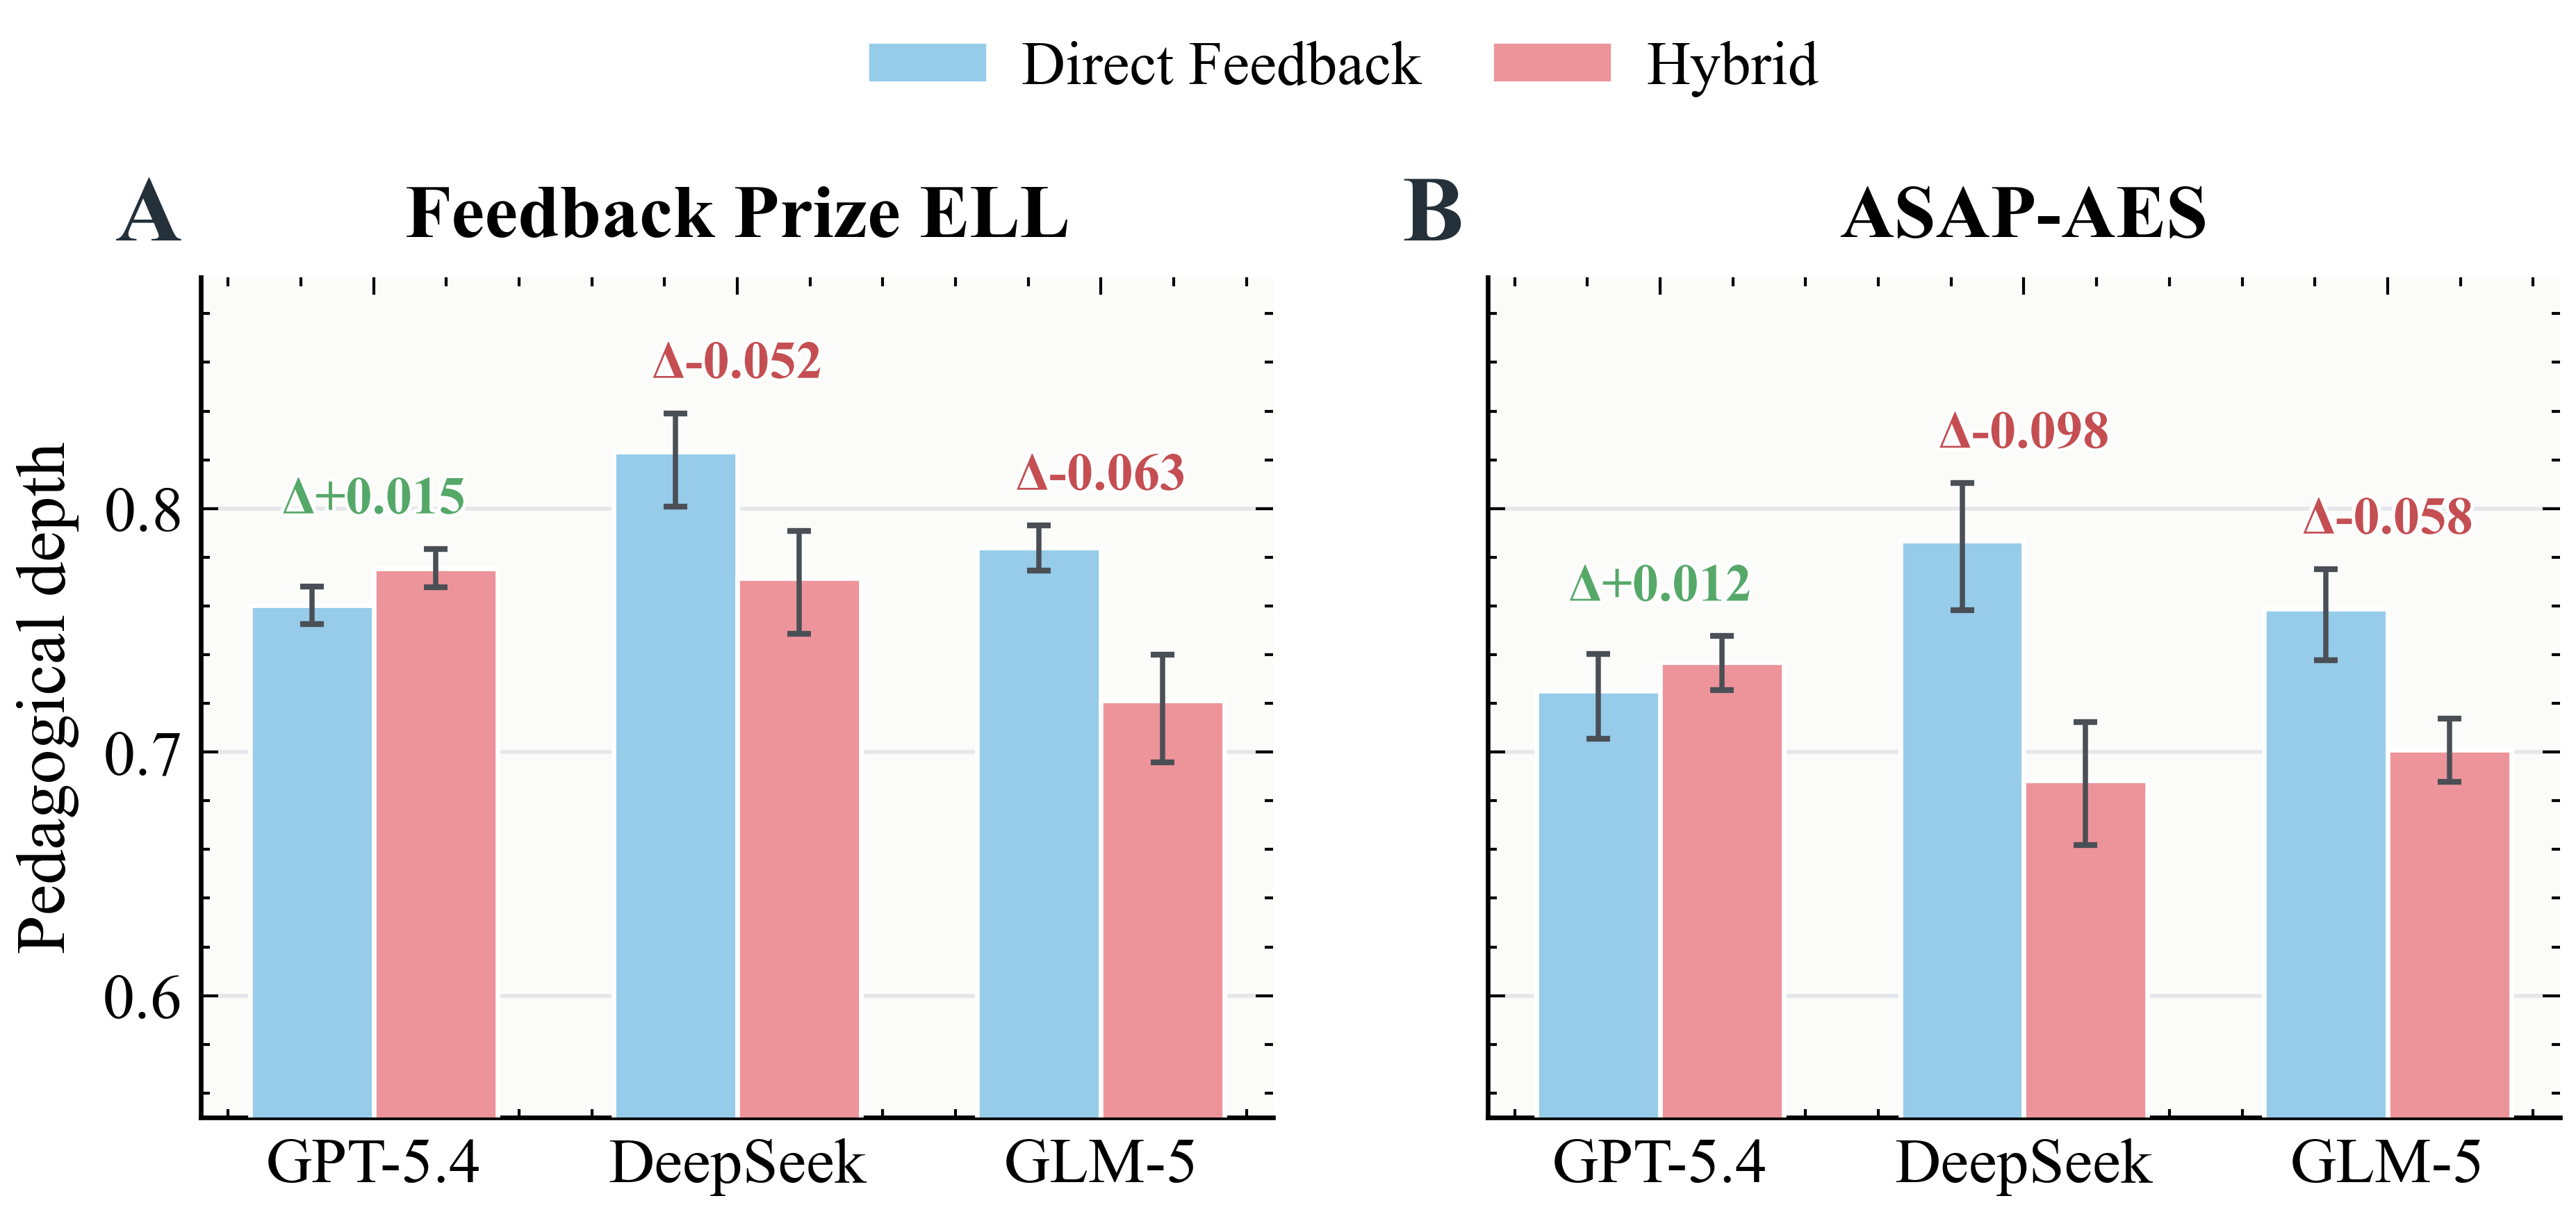
\includegraphics[width=\textwidth]{Fig/result_main_depth.png}
\caption{Cross-model pedagogical depth on ELL and ASAP-AES. Bars show mean depth; error bars show 95\% bootstrap intervals.}
\label{fig:main_depth_results}
\end{figure*}

\begin{figure*}[!t]
\centering
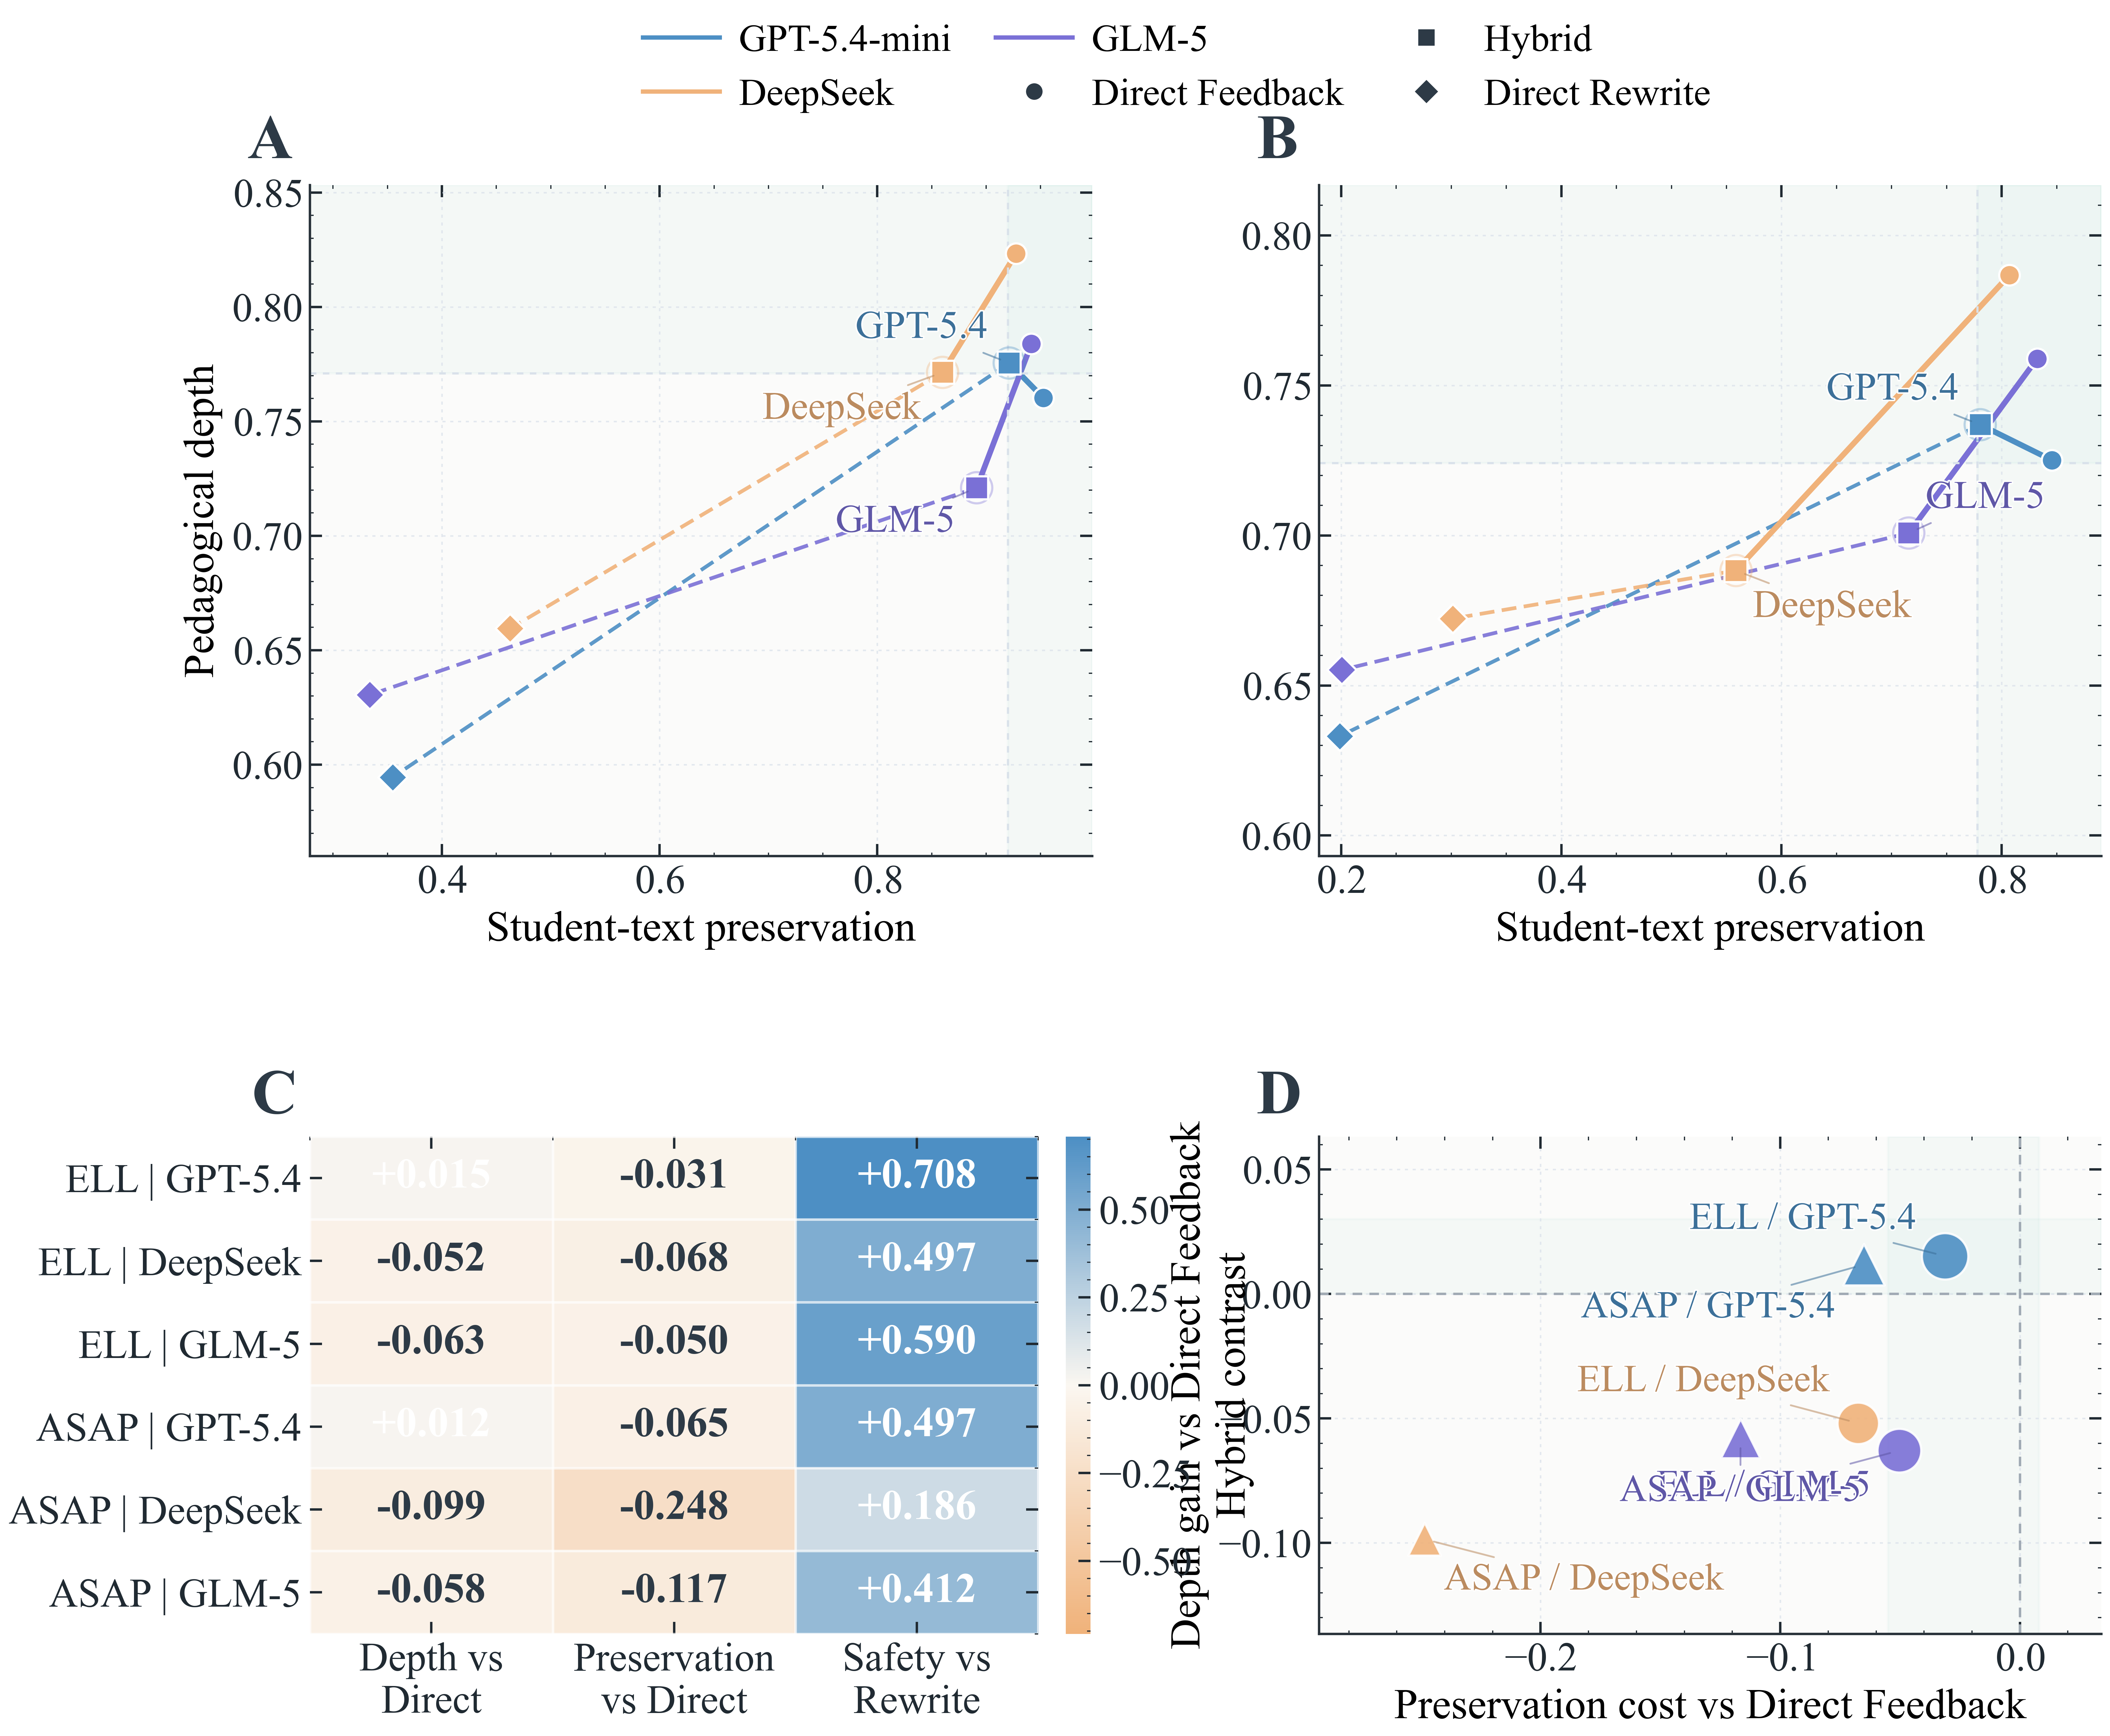
\includegraphics[width=\textwidth]{Fig/result_tradeoff_map.png}
\caption{Preservation and rewrite trade-offs across datasets and models. The figure contrasts direct rewrite, direct feedback, and hybrid in shared preservation--depth space.}
\label{fig:tradeoff_map}
\end{figure*}

\begin{table}[t]
\centering
\scriptsize
\caption{Blinded two-rater review on 24 items from three reported conditions. Higher is better except rewrite safety, where higher means less over-rewriting. Quadratic weighted $\kappa$ ranges from 0.943 to 1.000.}
\label{tab:human_review}
\begin{tabular*}{\linewidth}{@{\extracolsep{\fill}}lcccccc@{}}
\toprule
Condition & Act. & Clar. & Usef. & Cover. & Safety & Auto. \\
\midrule
Direct feedback & 3.33 & 3.50 & 3.00 & 3.44 & 4.00 & 3.28 \\
Hybrid & 3.00 & 3.11 & 2.83 & 2.78 & 2.78 & 3.06 \\
Rule-only & 1.00 & 1.50 & 1.00 & 1.00 & 5.00 & 1.00 \\
\bottomrule
\end{tabular*}
\end{table}

\paragraph{Human evaluation.}
The blinded 24-item human review reaches the same coarse ordering as the automatic analysis: direct feedback ranks above hybrid on usefulness, clarity, coverage, and rewrite safety, while both exceed rule-only. Given the small sample and three-condition scope, we treat these ratings as corroborative rather than dispositive.

\paragraph{Targeted refinement and repair.}
Follow-up analyses nonetheless show that the hybrid gap is not fixed. On failure-focused \texttt{GPT-5.4-mini} subsets, tighter exemplar control improved depth, preservation, and non-overwriting, and repair safeguards removed audited empty outputs and placeholder mentions; the detailed plots and robustness tables are therefore moved to the supplementary material. The practical implication is that part of the deficit comes from controllable prompt and pipeline hygiene rather than from the hybrid premise itself.

\section{Limitations and Ethical Considerations}

The paper makes benchmark claims, not classroom claims. Public learner-writing corpora are only proxies for authentic Chinese high-school use, automatic pedagogical scores are proxy metrics, and the 80-essay subsets mainly support effect direction and trade-off shape rather than final effect sizes. The human review is also small, covering only 24 items and three conditions.

The rule-tool layer imposes a quality ceiling and can introduce false positives, especially for learner-language phenomena not well covered by LanguageTool. Structured outputs can still hallucinate incorrect diagnoses or overconfident discourse advice, and the framework remains single-pass rather than dialogic. These technical risks translate into educational risk if feedback is treated as teacher replacement rather than teacher support.

\section{Conclusion}

Under matched benchmark conditions, a rule-tool and LLM hybrid can deliver pedagogically structured feedback, but its advantage over direct feedback is model-dependent rather than general. The paper's contribution is therefore protocol-level as much as model-level: it shows how to compare layered revision guidance, ownership preservation, rewrite safety, and schema reliability within one reproducible setup. The current evidence favors cautious deployment, further model-specific prompt calibration, larger benchmark runs, and eventual classroom studies that test whether these artifact-level gains translate into learning benefits.

\bibliographystyle{elsarticle-num}
\bibliography{references}

\end{document}
